\chapter{Fluxo de telas da aplicação}

As figuras a seguir ilustram o protótipo de telas da aplicação \emph{web}.

\begin{figure}[ht]
  \centering
    \caption{Protótipo da \emph{homepage} não autenticada e tela de entrada}
    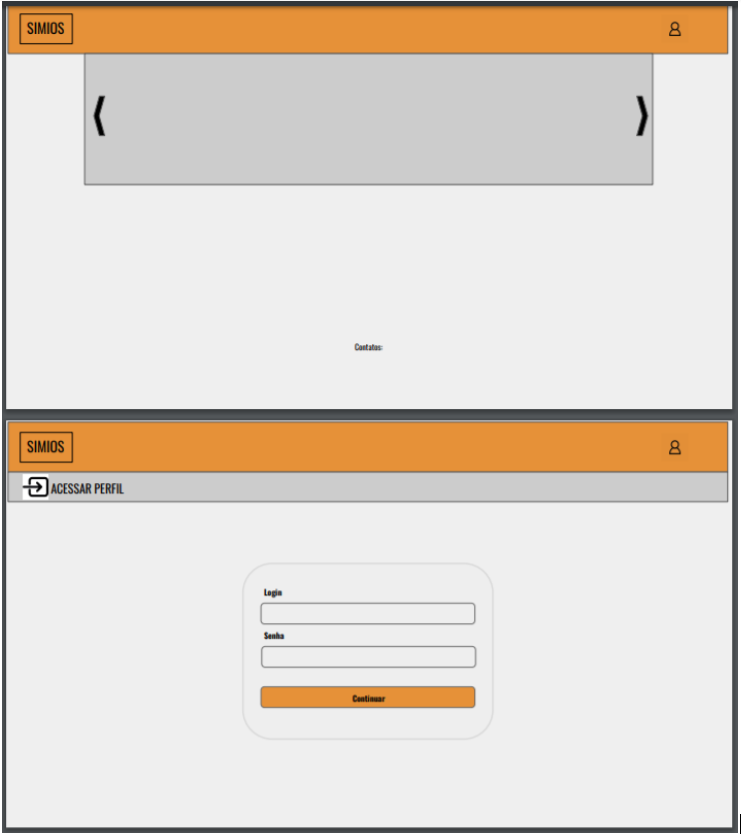
\includegraphics[scale=0.8]{fluxo-telas-1}
  \centerline{\small{Fonte: autores}}
\end{figure}

\begin{figure}[ht]
  \centering
    \caption{Protótipo da \emph{homepage} autenticada e da tela de listagem de usuários} 
    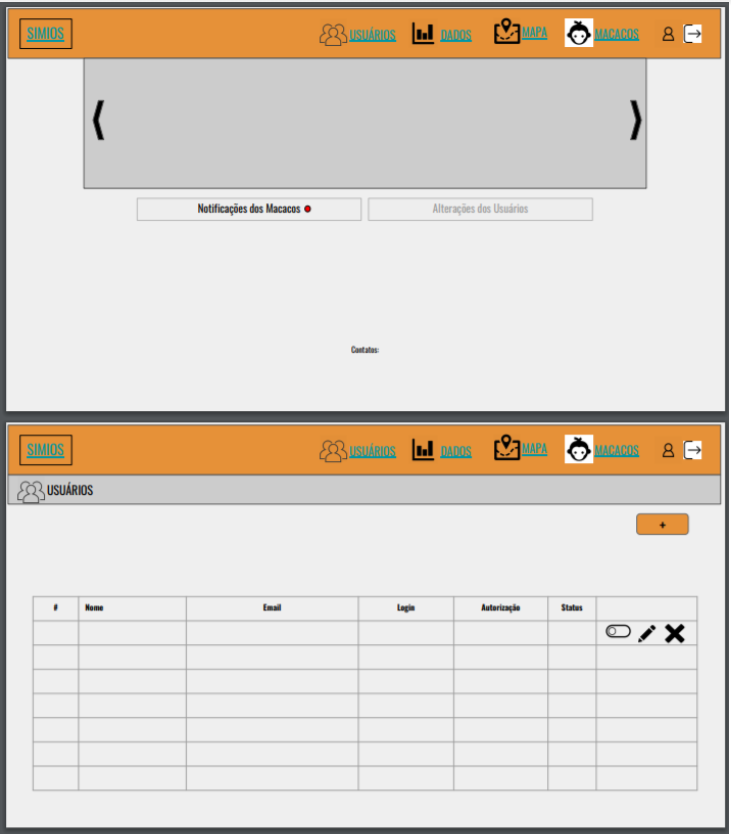
\includegraphics[scale=0.9]{fluxo-telas-2}
  \centerline{\small{Fonte: autores}}
\end{figure}

\begin{figure}[ht]
  \centering
    \caption{Protótipo das tela de cadastro de usuários e listagem de símios}
    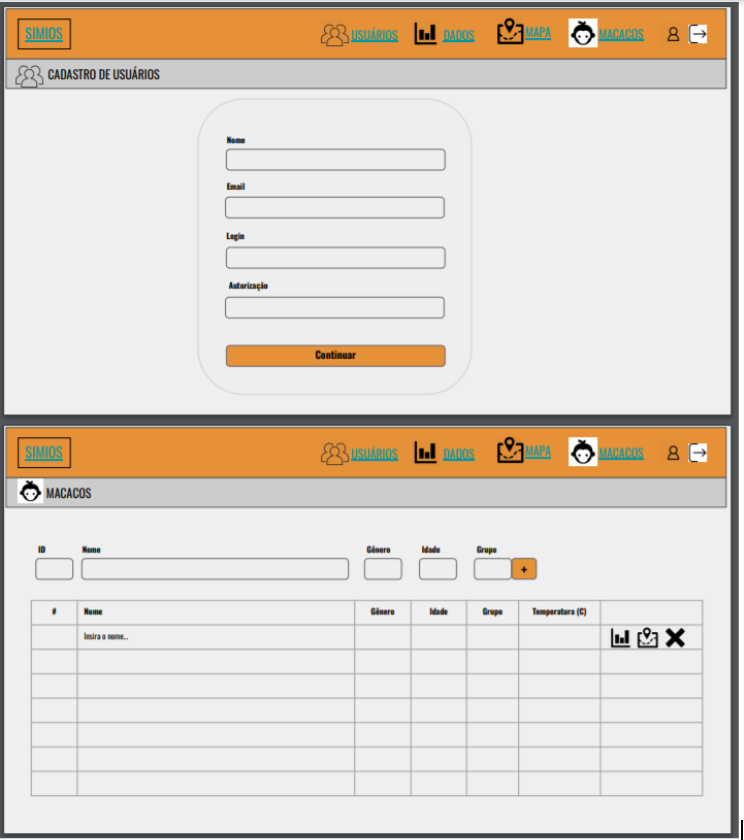
\includegraphics[scale=0.9]{fluxo-telas-3}
  \centerline{\small{Fonte: autores}}
\end{figure}

\begin{figure}[ht]
  \centering
    \caption{Protótipo da tela do mapa}
    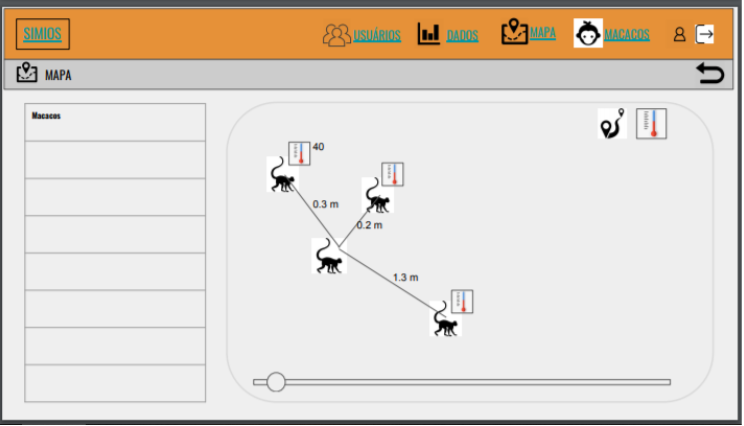
\includegraphics[scale=0.9]{fluxo-telas-4}
  \centerline{\small{Fonte: autores}}
\end{figure}
